\subsection{Goal-Based Investing model implementation}
\label{sec:gbi-model}

QWIM Version 1 is an explainable, client-driven retirement-planning workflow. It does not claim to forecast market returns or to provide online portfolio optimization. Instead, a client risk-tolerance category selects a predefined six-ETF policy, while confirmed plan assets translate that policy into dollar allocations. Figure~\ref{fig:gbi-workflow} summarizes the implementation pipeline.

\begin{table}[htbp]
\centering
\footnotesize
\caption{Client-data fields used in Goal-Based Investing Version 1.}
\label{tab:gbi-client-inputs}
\begin{tabular}{lp{0.55\linewidth}}
\toprule
Client field & Model use \\
\midrule
Risk tolerance & Selects one of five predefined risk-profile policies and its equity-risk band. \\
Taxable, tax-deferred and tax-free assets & Reported assets; the client confirms the amount allocated to the plan, which scales ETF dollar allocations. \\
Current age and retirement age & Define the retirement horizon and staged planning schedule. \\
Annual contribution & Pre-retirement contribution cash flow. \\
Social Security, pension, annuity and other income & Retirement-stage guaranteed-income cash flows, separate from invested wealth. \\
Essential, important and aspirational expenses & Priority spending schedules with descending shortfall protection. \\
\bottomrule
\end{tabular}
\end{table}

\begin{table}[htbp]
\centering
\footnotesize
\caption{Six-ETF strategic universe used by the GBI policies.}
\label{tab:gbi-etf-universe}
\begin{tabular}{lll}
\toprule
ETF & Asset role & Purpose in the policy \\
\midrule
BIL & Cash proxy & Liquidity and low-volatility allocation. \\
XLK & Equity sector & Technology equity exposure. \\
XLP & Equity sector & Defensive consumer-staples equity exposure. \\
AGG & Aggregate bonds & Core nominal bond exposure. \\
TIP & Inflation-linked bonds & Inflation-sensitive defensive exposure. \\
GLD & Gold & Diversifying real-asset exposure. \\
\bottomrule
\end{tabular}
\end{table}

\begin{table}[htbp]
\centering
\footnotesize
\caption{Risk-profile equity-allocation bands.}
\label{tab:gbi-risk-bands}
\begin{tabular}{lrr}
\toprule
Risk profile & Minimum equity & Maximum equity \\
\midrule
Conservative & 5% & 25% \\
Moderate Conservative & 25% & 40% \\
Moderate & 40% & 55% \\
Moderate Aggressive & 55% & 70% \\
Aggressive & 70% & 85% \\
\bottomrule
\end{tabular}
\end{table}


\begin{figure}[htbp]
  \centering
  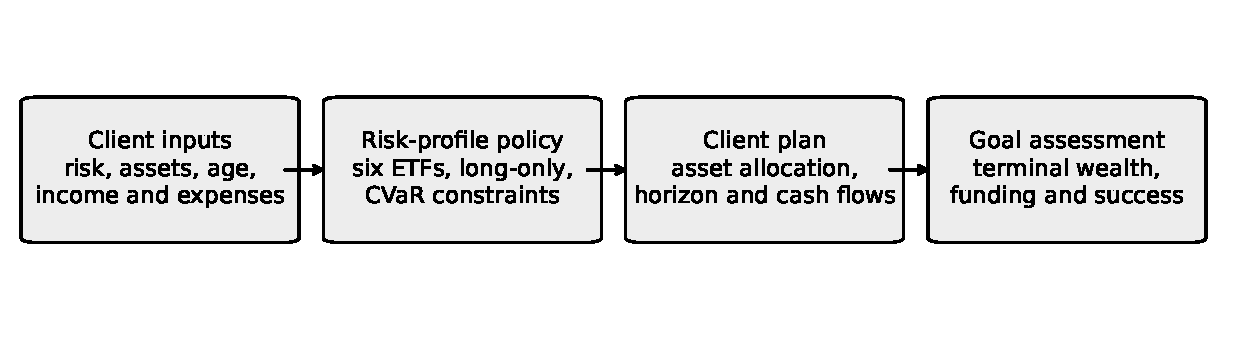
\includegraphics[width=0.98\linewidth]{model_implementation/figures/gbi_model_workflow.pdf}
  \caption{Client-data-to-goal-assessment workflow in GBI Version 1.}
  \label{fig:gbi-workflow}
\end{figure}

\subsubsection{Policy construction and historical evaluation}
Each policy is long-only and fully invested. The offline CVaR construction minimizes historical 95\% expected shortfall subject to the client risk-profile equity band and ETF caps. For research evaluation, the rolling baseline re-estimates policy weights from the preceding 36 monthly observations and applies them over the next quarter without future information. The evaluation includes 10bp one-way trading costs at quarterly rebalances. The Dashboard itself retains a versioned static policy so that it does not optimize separately for each client.

\begin{table}[htbp]
\centering
\footnotesize
\caption{Out-of-sample performance of six-ETF rolling CVaR policies (36-month trailing window).}
\label{tab:gbi-rolling-policy-36m}
\begin{tabular}{lrrrrrr}
\toprule
Risk profile & Annual return & Annual vol. & Sharpe & Max drawdown & ES (95\%) & Months \\
\midrule
Conservative & 5.12\% & 4.47\% & 1.14 & -8.13\% & 2.32\% & 59 \\
Moderate Conservative & 5.21\% & 5.62\% & 0.93 & -6.94\% & 2.75\% & 59 \\
Moderate & 9.11\% & 7.38\% & 1.22 & -6.85\% & 3.61\% & 59 \\
Moderate Aggressive & 9.33\% & 8.69\% & 1.07 & -6.39\% & 4.23\% & 59 \\
Aggressive & 10.20\% & 10.53\% & 0.98 & -12.26\% & 5.43\% & 59 \\
\bottomrule
\end{tabular}
\vspace{2pt}
\begin{minipage}{0.96\linewidth}
\footnotesize
Notes: Monthly walk-forward out-of-sample returns. Policies are re-optimized quarterly from the trailing 36-month window; 10bp one-way transaction costs are deducted at each rebalance. Annual return is CAGR; annual volatility and Sharpe use monthly data scaled by $\sqrt{12}$. Sharpe assumes a zero risk-free rate. ES is historical 95\% expected shortfall.
\end{minipage}
\end{table}


\paragraph{Interpretation and limitations.}
The rolling results are historical out-of-sample statistics, not forecasts or investment guarantees. The 95\% expected-shortfall estimate is based on a limited number of extreme monthly observations, and the 36-month window is a transparent research baseline rather than a claim of universal superiority. Client-level success probabilities are historical-bootstrap scenario frequencies and should be interpreted together with funding ratio and shortfall.

\subsubsection{Client goal assessment}
The selected policy is combined with confirmed plan assets, retirement horizon, annual contributions, income and priority spending. Goal success is evaluated over 2,000 historical-bootstrap terminal-wealth scenarios. The illustrative client results are reported in Table~\ref{tab:gbi-demo-goal-assessment}.

\begin{table}[htbp]
\centering
\footnotesize
\caption{Goal assessment for the illustrative Moderate client.}
\label{tab:gbi-demo-goal-assessment}
\begin{tabular}{lr}
\toprule
Metric & Value \\
\midrule
Confirmed plan assets & \$750,000 \\
Target retirement wealth & \$1,150,000 \\
Years to retirement & 5 \\
Annual contribution & \$25,000 \\
Selected risk profile & Moderate \\
Mean projected terminal wealth & \$1,216,109 \\
Funding ratio & 105.7% \\
Goal success probability & 66.6% \\
Shortfall / surplus & \$0 shortfall \\
\bottomrule
\end{tabular}
\vspace{2pt}
\begin{minipage}{0.92\linewidth}
\footnotesize
Notes: The illustrative client has \$750,000 of confirmed plan assets, a five-year horizon and \$25,000 annual contributions. Terminal wealth is evaluated over 2,000 historical-bootstrap monthly-return paths of the selected fixed Moderate policy; it is a scenario analysis, not a forecast.
\end{minipage}
\end{table}


\begin{figure}[htbp]
  \centering
  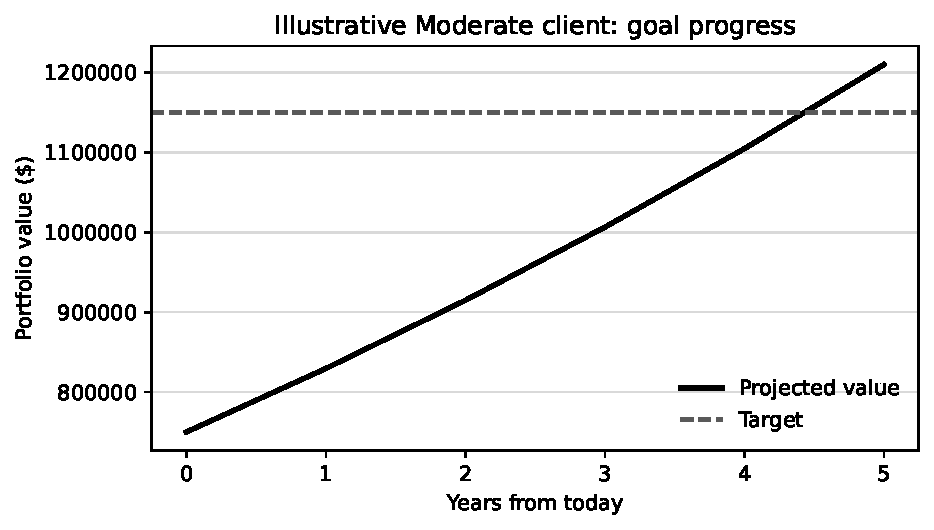
\includegraphics[width=0.82\linewidth]{model_implementation/figures/gbi_demo_client_goal_progress.pdf}
  \caption{Projected goal-progress path for the illustrative Moderate client.}
  \label{fig:gbi-demo-progress}
\end{figure}

\begin{figure}[htbp]
  \centering
  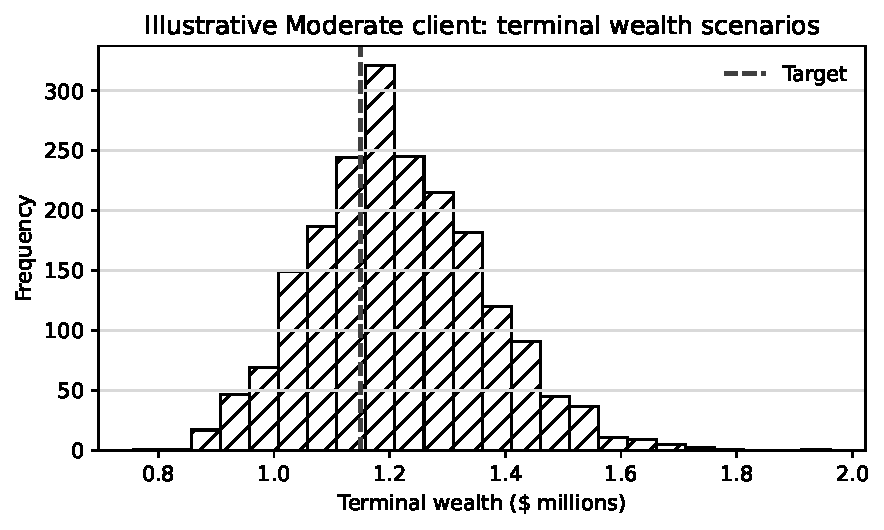
\includegraphics[width=0.82\linewidth]{model_implementation/figures/gbi_demo_client_terminal_distribution.pdf}
  \caption{Historical-bootstrap terminal-wealth distribution for the illustrative Moderate client.}
  \label{fig:gbi-demo-terminal}
\end{figure}
